
\chapter{Adaptive Control}
\label{chap:adaptive_control}

\begin{quote}
\textit{``The measure of intelligence is the ability to change.''} --- Albert Einstein
\end{quote}

\vspace{1em}

\noindent\textbf{Chapter Objectives:}
This chapter provides a comprehensive treatment of adaptive control systems. You will understand the historical development and motivation for adaptive control, gaining insight into why fixed controllers fail in environments with changing dynamics. The chapter covers the mathematical foundations of Model Reference Adaptive Control (MRAC) in depth, including the derivation of adaptation laws using both gradient descent (the MIT Rule) and Lyapunov stability methods. You will learn to implement self-tuning regulators and gain scheduling techniques for practical applications, apply adaptive control to motor control problems, and analyze the stability and convergence properties of adaptive systems.

%=============================================================================
\section{Historical Motivation: The Need for Adaptation}
\label{sec:adaptive_history}
%=============================================================================

The story of adaptive control is one of engineering necessity, mathematical innovation, and a cautionary tale about the gap between theory and practice. Understanding this history illuminates not only the development of the field but also the fundamental challenges that any adaptive control designer must confront.

\subsection{The Aircraft Problem: Where Fixed Controllers Fail}

In the early 1950s, aviation engineers faced an increasingly urgent problem. As aircraft became faster and flew at higher altitudes, the aerodynamic characteristics of these vehicles changed dramatically throughout their flight envelope. Consider the fundamental relationship governing aircraft dynamics:

The lift force on an aircraft wing is given by:
\begin{equation}
L = \frac{1}{2}\rho v^2 S C_L
\label{eq:lift}
\end{equation}
where $\rho$ is air density, $v$ is airspeed, $S$ is wing area, and $C_L$ is the lift coefficient. The dynamic pressure $q = \frac{1}{2}\rho v^2$ varies by orders of magnitude between takeoff and high-altitude cruise:

\begin{table}[H]
\centering
\caption{Variation of Dynamic Pressure Across Flight Envelope}
\label{tab:dynamic_pressure}
\begin{tabular}{lccc}
\toprule
\textbf{Flight Condition} & \textbf{Altitude (ft)} & \textbf{Speed (Mach)} & \textbf{Dynamic Pressure (psf)} \\
\midrule
Takeoff & 0 & 0.3 & 215 \\
Low-altitude cruise & 10,000 & 0.6 & 610 \\
High-altitude cruise & 40,000 & 0.85 & 270 \\
High-speed dash & 30,000 & 1.2 & 890 \\
\bottomrule
\end{tabular}
\end{table}

A controller designed for one flight condition---say, low-altitude cruise---would experience dramatically different plant dynamics at another condition. The transfer function of an aircraft's pitch dynamics takes the approximate form:
\begin{equation}
G(s) = \frac{K_\alpha(q, M)}{s^2 + 2\zeta(q,M)\omega_n(q,M)s + \omega_n^2(q,M)}
\label{eq:aircraft_dynamics}
\end{equation}
where all parameters depend on dynamic pressure $q$ and Mach number $M$. The gain $K_\alpha$ might vary by a factor of 10, while the natural frequency $\omega_n$ could change by a factor of 3.

\begin{historicalbox}[sharp corners]
\textbf{The X-15 Hypersonic Aircraft (1959-1968):} Perhaps no vehicle better illustrates the adaptive control challenge than the North American X-15. This rocket-powered research aircraft flew from the dense atmosphere at Edwards Air Force Base to the edge of space at 354,200 feet. During a typical flight, the dynamic pressure varied from 2,000 psf at low altitude to essentially zero in the upper atmosphere. The X-15 used an early form of gain scheduling, with the pilot manually adjusting stability augmentation system gains based on displayed flight conditions. Three X-15 aircraft made 199 flights, with pilots reporting significant workload managing the changing dynamics. This experience directly motivated the development of automated adaptive control systems.
\end{historicalbox}

\subsection{The MIT Rule: Birth of Adaptive Control (1958)}

The first systematic approach to adaptive control emerged from the MIT Instrumentation Laboratory (now Draper Laboratory) in the late 1950s. The research team, led by Whitaker, Yamron, and Kezer, proposed what became known as the \textbf{MIT Rule} in 1958.

The fundamental insight was elegant: if we define a tracking error between the actual plant output and a desired reference model output, we can adjust controller parameters to minimize this error using gradient descent.

\begin{keyconceptbox}[title=The MIT Rule Philosophy, sharp corners]
\textit{``If the system isn't behaving like the reference model, adjust the controller parameters in the direction that reduces the error.''}

This is formalized as:
\begin{equation}
\frac{d\theta}{dt} = -\gamma e \frac{\partial e}{\partial \theta}
\label{eq:mit_rule_intro}
\end{equation}
where $\theta$ represents controller parameters, $e$ is the tracking error, and $\gamma > 0$ is the adaptation gain.
\end{keyconceptbox}

The MIT Rule represented a paradigm shift: rather than designing a fixed controller for worst-case conditions (which would be conservative) or requiring continuous redesign (which would be impractical), the controller could continuously adjust itself to maintain performance.

The initial applications focused on autopilot systems, where the reference model represented the desired aircraft handling qualities---how the pilot wanted the aircraft to respond to stick inputs. The adaptive mechanism would adjust control gains so that the actual aircraft response matched this ideal model, regardless of flight condition.

\subsection{Lyapunov-Based Adaptation: Mathematical Rigor (1960s)}

While the MIT Rule provided an intuitive and often effective approach, it lacked formal stability guarantees. The adaptation law was based on minimizing an error cost function, but there was no proof that the closed-loop system would remain stable during the adaptation process.

This theoretical gap was addressed in the 1960s through the application of Lyapunov stability theory to adaptive control. The key figures in this development included Parks (1966), who applied Lyapunov methods to adaptive control, and Narendra and his colleagues, who developed systematic design procedures.

The Lyapunov approach reversed the design philosophy. The MIT Rule begins with an intuitive adaptation law and hopes for stability, whereas the Lyapunov approach starts with a stability requirement and derives the adaptation law from it.

By choosing an appropriate Lyapunov function that includes both the tracking error and parameter estimation error, one could \textit{derive} an adaptation law that guarantees $\dot{V} \leq 0$, ensuring stability. This was not merely an incremental improvement---it transformed adaptive control from an engineering heuristic to a mathematically rigorous discipline.

\begin{figure}[H]
\centering
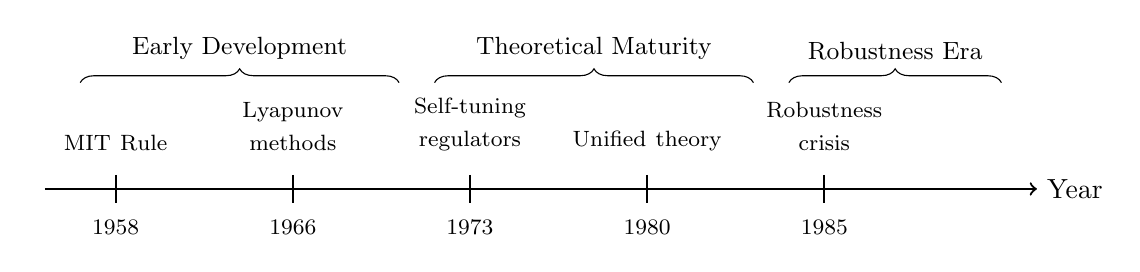
\begin{tikzpicture}[scale=0.9]
    % Timeline
    \draw[thick,->] (0,0) -- (14,0) node[right] {Year};

    % Major events
    \foreach \x/\year/\event in {
        1/1958/MIT Rule,
        3.5/1966/Lyapunov methods,
        6/1973/Self-tuning regulators,
        8.5/1980/Unified theory,
        11/1985/Robustness crisis
    } {
        \draw[thick] (\x,0.2) -- (\x,-0.2);
        \node[below] at (\x,-0.3) {\footnotesize \year};
        \node[above,text width=2cm,align=center] at (\x,0.4) {\footnotesize \event};
    }

    % Era labels
    \draw[decorate,decoration={brace,amplitude=5pt}] (0.5,1.5) -- (5,1.5)
        node[midway,above=5pt] {\small Early Development};
    \draw[decorate,decoration={brace,amplitude=5pt}] (5.5,1.5) -- (10,1.5)
        node[midway,above=5pt] {\small Theoretical Maturity};
    \draw[decorate,decoration={brace,amplitude=5pt}] (10.5,1.5) -- (13.5,1.5)
        node[midway,above=5pt] {\small Robustness Era};
\end{tikzpicture}
\caption{Timeline of major developments in adaptive control theory.}
\label{fig:timeline}
\end{figure}

\subsection{The Robustness Crisis: Rohrs' Counterexamples (1985)}

By the early 1980s, adaptive control theory had achieved considerable mathematical sophistication. Stability proofs existed for a variety of adaptive control architectures, and the field appeared mature. Then came a sobering demonstration that shook the foundations of the discipline.

In 1985, Rohrs, Valavani, Athans, and Stein published a landmark paper in \textit{IEEE Transactions on Automatic Control} titled ``Robustness of Continuous-Time Adaptive Control Algorithms in the Presence of Unmodeled Dynamics.'' Their findings were troubling.

\begin{warningbox}[title=Rohrs' Counterexample, sharp corners]
Rohrs et al. demonstrated that adaptive controllers which were \textit{provably stable} under ideal assumptions could become \textit{unstable} when unmodeled high-frequency dynamics were present, when output disturbances were added, or when both conditions occurred together. The instability could be dramatic, with bounded disturbances causing unbounded signals.
\end{warningbox}

The core issue was that all stability proofs relied on idealized assumptions. First, perfect model knowledge was assumed---the plant was taken to be exactly in the model class. Second, no unmodeled dynamics were considered, meaning high-frequency parasitic dynamics were ignored. Third, no disturbances were present, as the proofs assumed noise-free measurements.

Real systems violate all three assumptions. A DC motor has armature inductance (often neglected in simple models), sensors add noise, and mechanical systems have resonances at high frequencies.

The problem was particularly insidious because adaptive systems could appear to work well in simulation or initial testing, then fail catastrophically when deployed in conditions that excited the unmodeled dynamics.

\subsection{Resolution and Modern Perspective}

The robustness crisis did not kill adaptive control---instead, it transformed the field. Researchers developed modifications that restored robustness. The $\sigma$-modification adds a leakage term $-\sigma\theta$ to prevent parameter drift. The $\varepsilon_1$-modification introduces dead-zone modifications to stop adaptation when the error is small. Projection constrains parameters to remain in a known bounded region. Normalization scales signals to prevent unbounded growth.

These robustness modifications came at a cost: one could no longer prove asymptotic convergence of tracking error to zero. Instead, the error would converge to a small residual set. But this trade-off---perfect theoretical performance for practical robustness---is one that every practicing engineer should embrace.

\begin{historicalbox}[sharp corners]
\textbf{Legacy of the Robustness Crisis:} The Rohrs counterexamples served as a watershed moment for control theory broadly, not just adaptive control. They demonstrated the danger of mistaking mathematical elegance for engineering validity. Today, robustness analysis is considered essential for any advanced control design, and the gap between theoretical assumptions and practical reality is explicitly addressed rather than ignored.
\end{historicalbox}

%=============================================================================
\section{Modern Applications of Adaptive Control}
\label{sec:adaptive_applications}
%=============================================================================

While the theoretical foundations of adaptive control were established decades ago, modern applications continue to expand as computational power increases and new challenges emerge.

\subsection{Aerospace and Flight Control}

Adaptive control remains central to aerospace applications, where the original motivation persists. In commercial aircraft, fuel consumption changes the aircraft mass by 30\% or more during long flights. Military aircraft experience dynamics alterations due to weapons release, battle damage, and configuration changes. Spacecraft undergo mass property changes from fuel depletion and appendage deployment. Unmanned aerial vehicles (UAVs) require adaptation to handle payload variations and icing conditions.

NASA's Intelligent Flight Control System (IFCS) demonstrated neural network-based adaptive control on the F-15 ACTIVE research aircraft, showing the ability to maintain control even with significant control surface failures.

\subsection{Robotics and Manufacturing}

Modern robots face continuously changing conditions that classical fixed controllers handle poorly. Payload variation requires different gains when a robot arm carries different loads. Wear and degradation cause joint friction and gear backlash to change over time. Human-robot interaction demands adaptive compliance when robots make contact with humans. Learning from demonstration requires adapting to new tasks shown by operators.

\subsection{Process Industry}

Chemical and manufacturing processes exhibit slow parameter variations that motivate adaptive approaches. Catalyst deactivation causes reaction rates to decrease over weeks or months. Fouling degrades heat exchanger coefficients as deposits accumulate. Raw material variation affects process dynamics as feed composition changes. Seasonal changes alter heat transfer as cooling water temperature varies.

Self-tuning PID controllers are widely deployed in process industries, automatically adjusting gains to maintain performance as conditions drift.

\subsection{Biomedical Applications}

Adaptive control has found growing application in medical devices. Artificial pancreas systems must adapt insulin delivery to varying patient sensitivity. Anesthesia control systems accommodate drug sensitivity that varies between patients and during surgery. EMG-controlled prosthetic limbs adapt to user patterns over time. Rehabilitation robots adjust therapy assistance based on patient progress.

\subsection{Automotive Systems}

Modern vehicles contain numerous adaptive control systems. Engine control units adapt fuel injection to altitude, temperature, and fuel quality. Transmission control systems adjust shift patterns based on driver behavior. Active suspension systems adapt damping to road conditions and vehicle load. Autonomous vehicles adapt their control strategies to road surface conditions and environmental factors.

%=============================================================================
\section{Mathematical Foundations of Adaptive Control}
\label{sec:adaptive_math}
%=============================================================================

We now develop the mathematical framework for adaptive control, progressing from simple intuitive approaches to rigorous Lyapunov-based designs.

\subsection{The Adaptive Control Problem}

Consider a plant with unknown or time-varying parameters:
\begin{equation}
\dot{x} = A(\theta)x + B(\theta)u, \qquad y = Cx
\label{eq:uncertain_plant}
\end{equation}
where $\theta \in \mathbb{R}^p$ represents the unknown parameter vector. The control objective is to make the output $y$ track a reference signal $r(t)$ despite the uncertainty in $\theta$.

The key insight of adaptive control is to treat the unknown parameters as additional states to be estimated, then use these estimates in the controller:
\begin{equation}
u = K(\hat{\theta})x + L(\hat{\theta})r
\label{eq:adaptive_controller}
\end{equation}
where $\hat{\theta}$ is the current parameter estimate. The adaptation mechanism updates $\hat{\theta}$ based on observed system behavior.

\subsection{Model Reference Adaptive Control (MRAC)}

\subsubsection{Reference Model Concept}

In MRAC, we specify desired closed-loop behavior through a reference model:
\begin{equation}
\dot{x}_m = A_m x_m + B_m r
\label{eq:reference_model}
\end{equation}
where $A_m$ is Hurwitz (stable), and the model represents ideal behavior we want the plant to achieve.

\begin{keyconceptbox}[title=Reference Model Selection, sharp corners]
The reference model should satisfy three essential criteria. First, it must be stable, with $A_m$ having all eigenvalues in the left half-plane. Second, the model must be achievable, meaning the plant must be capable of matching the model behavior. Third, the model should exhibit the desired behavior, with its response matching specifications such as rise time and overshoot.
\end{keyconceptbox}

For a first-order plant $\dot{y} = -a y + b u$ where we want first-order reference behavior $\dot{y}_m = -a_m y_m + b_m r$, the controller takes the form:
\begin{equation}
u = \theta_1 r + \theta_2 y
\label{eq:mrac_first_order}
\end{equation}

If we knew the true parameters $a$ and $b$, we would select:
\begin{equation}
\theta_1^* = \frac{b_m}{b}, \qquad \theta_2^* = \frac{a - a_m}{b}
\label{eq:ideal_params}
\end{equation}

Since $a$ and $b$ are unknown, we use adaptive estimates $\hat{\theta}_1$ and $\hat{\theta}_2$ that are updated online.

\subsubsection{MRAC Block Diagram}

\begin{figure}[H]
\centering
\begin{tikzpicture}[
    block/.style={draw, rectangle, minimum height=1cm, minimum width=1.5cm},
    sum/.style={draw, circle, inner sep=2pt},
    >=latex
]
    % Reference model branch
    \node[block] (refmodel) at (0,3) {Reference Model};
    \node[left=1cm of refmodel] (r1) {$r$};
    \draw[->] (r1) -- (refmodel);
    \node[right=1cm of refmodel] (ym) {$y_m$};
    \draw[->] (refmodel) -- (ym);

    % Main control loop
    \node[sum] (sum1) at (0,0) {$+$};
    \node[block] (controller) at (2.5,0) {Controller};
    \node[block] (plant) at (5.5,0) {Plant};
    \node[right=1cm of plant] (y) {$y$};
    \node[left=1cm of sum1] (r2) {$r$};

    \draw[->] (r2) -- node[above,pos=0.3] {} (sum1);
    \draw[->] (sum1) -- (controller);
    \draw[->] (controller) -- node[above] {$u$} (plant);
    \draw[->] (plant) -- (y);

    % Feedback
    \draw[->] (7,0) -- (7,-1.5) -- (0,-1.5) -- (sum1);
    \node at (0.3,-0.3) {\small $-$};

    % Adaptation mechanism
    \node[block, minimum width=2.5cm] (adapt) at (3.5,-3) {Adaptation Mechanism};

    % Error signal
    \node[sum] (error) at (8,1.5) {$-$};
    \draw[->] (7,0) -- (7,1.5) -- (error);
    \draw[->] (ym) -- (3,3) -- (3,1.5) -- (error);
    \node at (8.3,1.2) {\small $+$};

    \node[right=0.5cm of error] (e) {$e$};
    \draw[->] (error) -- (e);

    % Connections to adaptation
    \draw[->] (9,1.5) -- (9,-3) -- (adapt);
    \draw[->] (6.5,0) -- (6.5,-2) -- (6,-2) -- (6,-3) -- (adapt);
    \draw[->] (adapt) -- (3.5,-1) -- (2.5,-1) -- (controller);

    \node at (4,-1.3) {\small $\hat{\theta}$};
\end{tikzpicture}
\caption{Block diagram of Model Reference Adaptive Control (MRAC). The adaptation mechanism adjusts controller parameters $\hat{\theta}$ to minimize the tracking error $e = y - y_m$.}
\label{fig:mrac_block}
\end{figure}

\subsection{MIT Rule Derivation}

The MIT Rule provides an intuitive approach to deriving adaptation laws based on gradient descent.

\subsubsection{Cost Function Approach}

Define a cost function based on tracking error:
\begin{equation}
J(\theta) = \frac{1}{2}e^2 = \frac{1}{2}(y - y_m)^2
\label{eq:mit_cost}
\end{equation}

To minimize $J$, we update parameters in the negative gradient direction:
\begin{equation}
\frac{d\theta}{dt} = -\gamma \frac{\partial J}{\partial \theta} = -\gamma e \frac{\partial e}{\partial \theta}
\label{eq:mit_rule_derivation}
\end{equation}

The term $\frac{\partial e}{\partial \theta}$ is called the \textbf{sensitivity derivative}. It measures how the error changes when parameters are perturbed.

\subsubsection{Application to First-Order System}

Consider the first-order plant:
\begin{equation}
\dot{y} = -ay + bu
\label{eq:first_order_plant}
\end{equation}
with unknown positive parameters $a$ and $b$. The reference model is:
\begin{equation}
\dot{y}_m = -a_m y_m + b_m r
\label{eq:first_order_ref}
\end{equation}

Using the controller $u = \hat{\theta}_1 r + \hat{\theta}_2 y$, the closed-loop plant becomes:
\begin{equation}
\dot{y} = -(a - b\hat{\theta}_2)y + b\hat{\theta}_1 r
\label{eq:closed_loop_first}
\end{equation}

For the plant to match the reference model, we need:
\begin{equation}
a - b\hat{\theta}_2 = a_m, \qquad b\hat{\theta}_1 = b_m
\label{eq:matching_conditions}
\end{equation}

\textbf{Deriving the sensitivity derivatives:}

From the closed-loop dynamics, in steady state (assuming slow adaptation), the output satisfies:
\begin{equation}
y = \frac{b\hat{\theta}_1}{a - b\hat{\theta}_2}r \quad \text{(for constant } r\text{)}
\label{eq:steady_state}
\end{equation}

Taking partial derivatives:
\begin{equation}
\frac{\partial y}{\partial \hat{\theta}_1} \approx \frac{b}{a - b\hat{\theta}_2}r \approx \frac{y_m}{\hat{\theta}_1}
\label{eq:sensitivity1}
\end{equation}
\begin{equation}
\frac{\partial y}{\partial \hat{\theta}_2} \approx \frac{b^2\hat{\theta}_1}{(a - b\hat{\theta}_2)^2}r \cdot y \approx \frac{y \cdot y_m}{\hat{\theta}_1}
\label{eq:sensitivity2}
\end{equation}

In practice, we often approximate:
\begin{equation}
\frac{\partial e}{\partial \hat{\theta}_1} \approx -y_m, \qquad \frac{\partial e}{\partial \hat{\theta}_2} \approx -y \cdot \text{sgn}(b)
\label{eq:practical_sensitivity}
\end{equation}

This leads to the MIT Rule adaptation laws:
\begin{equation}
\boxed{
\dot{\hat{\theta}}_1 = \gamma_1 e \cdot y_m, \qquad \dot{\hat{\theta}}_2 = \gamma_2 e \cdot y
}
\label{eq:mit_adaptation_laws}
\end{equation}

\begin{remark}
The MIT Rule requires knowledge of $\text{sgn}(b)$, the sign of the control gain. This is a minimal assumption---we must at least know whether increasing control increases or decreases the output.
\end{remark}

\subsection{Lyapunov-Based Adaptive Control}

The Lyapunov approach provides stability guarantees that the MIT Rule lacks. The methodology proceeds as follows: first, define the error dynamics relating the tracking error to parameter estimation errors; second, choose a Lyapunov function that includes both state error and parameter error terms; and third, derive the adaptation law that ensures $\dot{V} \leq 0$.

\subsubsection{Error Dynamics}

Let $\tilde{\theta} = \hat{\theta} - \theta^*$ denote the parameter estimation error, where $\theta^*$ are the ideal parameters. The tracking error dynamics can be written as:
\begin{equation}
\dot{e} = A_m e + B \phi(x,r)^T \tilde{\theta}
\label{eq:error_dynamics}
\end{equation}
where $\phi(x,r)$ is a regression vector and $B$ is the control input matrix.

\subsubsection{Lyapunov Function Construction}

Choose the Lyapunov function candidate:
\begin{equation}
V(e, \tilde{\theta}) = e^T P e + \tilde{\theta}^T \Gamma^{-1} \tilde{\theta}
\label{eq:lyapunov_candidate}
\end{equation}
where $P > 0$ satisfies the Lyapunov equation $A_m^T P + P A_m = -Q$ for some $Q > 0$, and $\Gamma > 0$ is a diagonal matrix of adaptation gains.

\subsubsection{Derivative Calculation}

Taking the time derivative:
\begin{align}
\dot{V} &= \dot{e}^T P e + e^T P \dot{e} + 2\tilde{\theta}^T \Gamma^{-1} \dot{\tilde{\theta}} \nonumber \\
&= e^T(A_m^T P + P A_m)e + 2e^T P B \phi^T \tilde{\theta} + 2\tilde{\theta}^T \Gamma^{-1} \dot{\hat{\theta}} \nonumber \\
&= -e^T Q e + 2\tilde{\theta}^T(\phi B^T P e + \Gamma^{-1} \dot{\hat{\theta}})
\label{eq:V_dot}
\end{align}

\subsubsection{Adaptation Law Derivation}

To make $\dot{V} \leq 0$, we choose the adaptation law:
\begin{equation}
\boxed{
\dot{\hat{\theta}} = -\Gamma \phi B^T P e
}
\label{eq:lyapunov_adaptation}
\end{equation}

This cancels the indefinite term, yielding:
\begin{equation}
\dot{V} = -e^T Q e \leq 0
\label{eq:V_dot_final}
\end{equation}

\begin{theorem}[Stability of Lyapunov-Based MRAC]
\label{thm:mrac_stability}
Consider the adaptive system with the adaptation law (\ref{eq:lyapunov_adaptation}). Then all signals in the closed-loop system are bounded, the tracking error $e(t) \to 0$ as $t \to \infty$, and the parameter estimates $\hat{\theta}(t)$ remain bounded.
\end{theorem}

\begin{proof}
Since $\dot{V} \leq 0$ and $V > 0$, the function $V(t)$ is non-increasing and bounded below by zero. Therefore, $V(t)$ converges to a limit, implying both $e$ and $\tilde{\theta}$ are bounded.

From $\dot{V} = -e^T Q e$, integrating from $0$ to $T$:
\begin{equation}
\int_0^T e^T Q e \, dt = V(0) - V(T) \leq V(0) < \infty
\label{eq:integral_bound}
\end{equation}

Thus $e \in \mathcal{L}_2$. Since $e$ and $\dot{e}$ are bounded (from bounded signals and the error dynamics), Barbalat's lemma implies $e(t) \to 0$ as $t \to \infty$.
\end{proof}

\begin{remark}[Parameter Convergence]
Note that Theorem \ref{thm:mrac_stability} does \textbf{not} guarantee $\tilde{\theta}(t) \to 0$. The parameters converge to values that produce zero tracking error, but these need not be the true plant parameters unless a \textbf{persistence of excitation} condition is satisfied.
\end{remark}

\subsubsection{Detailed Example: First-Order MRAC Design}

Consider the first-order plant $\dot{y} = -ay + bu$ with $a, b$ unknown but $b > 0$. Design an MRAC with reference model $\dot{y}_m = -a_m y_m + b_m r$.

\textbf{Step 1: Controller structure}
\begin{equation}
u = \hat{\theta}_1 r + \hat{\theta}_2 y
\end{equation}

\textbf{Step 2: Error dynamics}

Substituting the controller into the plant:
\begin{equation}
\dot{y} = -ay + b(\hat{\theta}_1 r + \hat{\theta}_2 y) = -(a - b\hat{\theta}_2)y + b\hat{\theta}_1 r
\end{equation}

With ideal parameters $\theta_1^* = b_m/b$ and $\theta_2^* = (a-a_m)/b$:
\begin{equation}
\dot{e} = \dot{y} - \dot{y}_m = -a_m e + b\tilde{\theta}_1 r + b\tilde{\theta}_2 y
\end{equation}

\textbf{Step 3: Lyapunov function}

Choose $V = \frac{1}{2}e^2 + \frac{b}{2\gamma_1}\tilde{\theta}_1^2 + \frac{b}{2\gamma_2}\tilde{\theta}_2^2$

Taking the derivative:
\begin{align}
\dot{V} &= e\dot{e} + \frac{b}{\gamma_1}\tilde{\theta}_1\dot{\hat{\theta}}_1 + \frac{b}{\gamma_2}\tilde{\theta}_2\dot{\hat{\theta}}_2 \nonumber \\
&= -a_m e^2 + be\tilde{\theta}_1 r + be\tilde{\theta}_2 y + \frac{b}{\gamma_1}\tilde{\theta}_1\dot{\hat{\theta}}_1 + \frac{b}{\gamma_2}\tilde{\theta}_2\dot{\hat{\theta}}_2 \nonumber \\
&= -a_m e^2 + b\tilde{\theta}_1\left(er + \frac{\dot{\hat{\theta}}_1}{\gamma_1}\right) + b\tilde{\theta}_2\left(ey + \frac{\dot{\hat{\theta}}_2}{\gamma_2}\right)
\end{align}

\textbf{Step 4: Adaptation law}

Choosing:
\begin{equation}
\dot{\hat{\theta}}_1 = -\gamma_1 e r, \qquad \dot{\hat{\theta}}_2 = -\gamma_2 e y
\end{equation}

yields $\dot{V} = -a_m e^2 \leq 0$, guaranteeing stability.

\subsection{Self-Tuning Regulators}

Self-Tuning Regulators (STR) take a different approach from MRAC: rather than forcing the plant to match a reference model, they explicitly identify plant parameters and update the controller accordingly.

\subsubsection{STR Architecture}

\begin{figure}[H]
\centering
\begin{tikzpicture}[
    block/.style={draw, rectangle, minimum height=1cm, minimum width=2cm},
    >=latex
]
    % Plant
    \node[block] (plant) at (6,0) {Plant};
    \node[left=1cm of plant] (u) {$u$};
    \node[right=1cm of plant] (y) {$y$};
    \draw[->] (u) -- (plant);
    \draw[->] (plant) -- (y);

    % Parameter estimator
    \node[block, minimum width=2.5cm] (estimator) at (6,-2.5) {Parameter Estimator};

    % Controller design
    \node[block, minimum width=2.5cm] (design) at (0,-2.5) {Controller Design};

    % Controller
    \node[block] (controller) at (0,0) {Controller};

    % Reference
    \node[left=1cm of controller] (r) {$r$};
    \draw[->] (r) -- (controller);
    \draw[->] (controller) -- (u);

    % Connections
    \draw[->] (5,0) -- (5,-1.5) -- (estimator);
    \draw[->] (7.5,0) -- (7.5,-2.5) -- (estimator);
    \draw[->] (estimator) -- node[below] {$\hat{\theta}$} (design);
    \draw[->] (design) -- node[left] {Controller params} (controller);

    % Labels
    \node at (4.5,-1.2) {\small $u$};
    \node at (7.8,-1.2) {\small $y$};
\end{tikzpicture}
\caption{Self-Tuning Regulator architecture: explicit separation of identification and control.}
\label{fig:str_block}
\end{figure}

\subsubsection{Recursive Least Squares Identification}

For a discrete-time ARX model:
\begin{equation}
y(k) = \phi(k)^T \theta + e(k)
\label{eq:arx_model}
\end{equation}
where $\phi(k) = [-y(k-1), \ldots, -y(k-n_a), u(k-1), \ldots, u(k-n_b)]^T$ is the regression vector.

The Recursive Least Squares (RLS) algorithm updates the parameter estimate:
\begin{align}
K(k) &= \frac{P(k-1)\phi(k)}{\lambda + \phi(k)^T P(k-1)\phi(k)} \label{eq:rls_gain}\\
\hat{\theta}(k) &= \hat{\theta}(k-1) + K(k)[y(k) - \phi(k)^T\hat{\theta}(k-1)] \label{eq:rls_update}\\
P(k) &= \frac{1}{\lambda}\left[P(k-1) - K(k)\phi(k)^T P(k-1)\right] \label{eq:rls_covariance}
\end{align}
where $\lambda \in (0,1]$ is a forgetting factor that allows tracking of time-varying parameters.

\subsubsection{Certainty Equivalence Principle}

Given the estimated parameters $\hat{\theta}$, the controller is designed as if $\hat{\theta}$ were the true parameters. This is called the \textbf{certainty equivalence principle}.

For a minimum variance controller, the control law becomes:
\begin{equation}
u(k) = \frac{1}{\hat{b}_1}\left[r(k+d) + \sum_{i=1}^{n_a} \hat{a}_i y(k+1-i) - \sum_{i=2}^{n_b} \hat{b}_i u(k+1-i)\right]
\label{eq:mv_control}
\end{equation}
where $d$ is the system delay.

\subsection{Gain Scheduling}

Gain scheduling is the simplest and most widely used form of adaptive control. It uses pre-computed controllers for different operating conditions, interpolating between them in real-time.

\subsubsection{Design Procedure}

\begin{algorithm}
\caption{Gain Scheduling Design Procedure}
\begin{algorithmic}[1]
\State \textbf{Identify scheduling variables:} Select measurable variables that correlate with parameter changes (e.g., altitude, speed, temperature)
\State \textbf{Define operating points:} Select representative conditions spanning the operating envelope
\State \textbf{Design local controllers:} At each operating point, linearize the plant and design an optimal controller
\State \textbf{Implement interpolation:} Create smooth transitions between controllers based on the scheduling variable
\State \Return Gain-scheduled controller with interpolation lookup table
\end{algorithmic}
\end{algorithm}

\subsubsection{Linear Interpolation}

For a single scheduling variable $\rho$ and two operating points $\rho_1$ and $\rho_2$:
\begin{equation}
K(\rho) = \frac{\rho_2 - \rho}{\rho_2 - \rho_1}K_1 + \frac{\rho - \rho_1}{\rho_2 - \rho_1}K_2
\label{eq:gain_interpolation}
\end{equation}

For multiple scheduling variables, multi-dimensional interpolation (e.g., bilinear, tensor product) is used.

\begin{figure}[H]
\centering
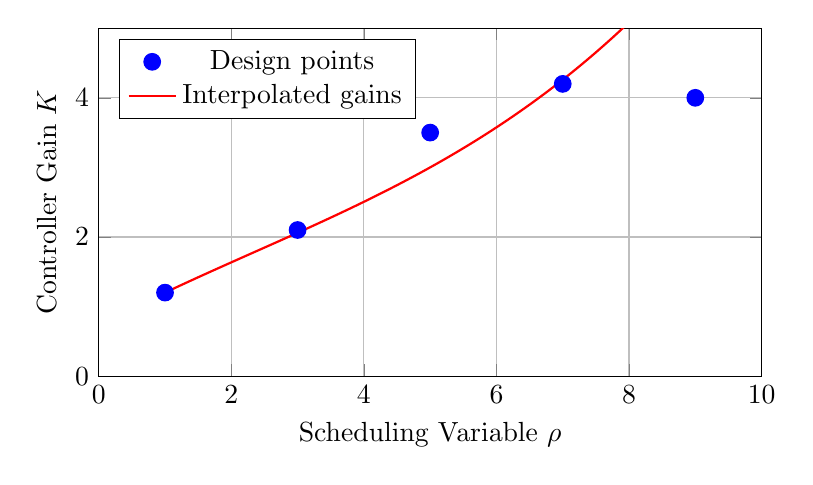
\begin{tikzpicture}
\begin{axis}[
    width=10cm, height=6cm,
    xlabel={Scheduling Variable $\rho$},
    ylabel={Controller Gain $K$},
    xmin=0, xmax=10,
    ymin=0, ymax=5,
    grid=major,
    legend pos=north west
]
    % Design points
    \addplot[only marks, mark=*, mark size=3pt, blue] coordinates {
        (1,1.2) (3,2.1) (5,3.5) (7,4.2) (9,4.0)
    };

    % Interpolated curve
    \addplot[smooth, thick, red, domain=1:9, samples=50] {
        1.2 + 0.45*(x-1) - 0.02*(x-1)^2 + 0.005*(x-1)^3
    };

    \legend{Design points, Interpolated gains}
\end{axis}
\end{tikzpicture}
\caption{Gain scheduling: controller gains interpolated between design operating points.}
\label{fig:gain_scheduling}
\end{figure}

\subsubsection{Stability Considerations}

Gain scheduling provides no formal stability guarantees during transitions. Sufficient conditions for stability include operating points close enough that interpolated controllers stabilize intermediate plants, scheduling variables that change slowly compared to closed-loop dynamics, and the use of LPV (Linear Parameter-Varying) design methods that explicitly account for parameter rates.

\subsection{Robustness Modifications}

The robustness crisis of the 1980s led to several modifications of basic adaptive laws:

\subsubsection{$\sigma$-Modification (Leakage)}

Add a damping term to prevent parameter drift:
\begin{equation}
\dot{\hat{\theta}} = -\Gamma \phi B^T P e - \sigma \hat{\theta}
\label{eq:sigma_mod}
\end{equation}
where $\sigma > 0$ is small. This pulls parameters toward zero, preventing drift when the error is small or when unmodeled dynamics cause persistent excitation.

\subsubsection{$e_1$-Modification (Dead Zone)}

Stop adaptation when error is below a threshold:
\begin{equation}
\dot{\hat{\theta}} = \begin{cases}
-\Gamma \phi B^T P e & \text{if } |e| > e_1 \\
0 & \text{if } |e| \leq e_1
\end{cases}
\label{eq:e1_mod}
\end{equation}

\subsubsection{Projection}

Constrain parameters to a known bounded set $\Omega$:
\begin{equation}
\dot{\hat{\theta}} = \text{Proj}(-\Gamma \phi B^T P e)
\label{eq:projection}
\end{equation}
where the projection operator prevents $\hat{\theta}$ from leaving $\Omega$.

%=============================================================================
\section{Practical Experiment: Adaptive Motor Control}
\label{sec:adaptive_experiment}
%=============================================================================

\begin{experimentbox}[title=Adaptive DC Motor Speed Control with Variable Load, sharp corners]
\textbf{Objective:} Demonstrate that an adaptive controller maintains performance under varying load conditions where a fixed controller fails.

\textbf{Time Required:} 3-4 hours

\textbf{Difficulty:} Intermediate
\end{experimentbox}

\subsection{Experimental Setup}

\subsubsection{Hardware Requirements}

\begin{table}[H]
\centering
\caption{Hardware Components for Adaptive Motor Control Experiment}
\begin{tabular}{ll}
\toprule
\textbf{Component} & \textbf{Specification} \\
\midrule
Microcontroller & Arduino Uno or Mega \\
Motor & DC motor with encoder (e.g., Pololu 37D gearmotor) \\
Motor driver & L298N H-bridge or similar \\
Power supply & 12V, 2A recommended \\
Load mechanism & Rotary disc with mounting points for weights \\
Calibrated weights & 10g, 20g, 50g, 100g set \\
Data acquisition & Oscilloscope or data logging capability \\
\bottomrule
\end{tabular}
\end{table}

\subsubsection{System Schematic}

\begin{figure}[H]
\centering
\begin{circuitikz}[scale=0.8]
    % Arduino
    \draw (0,0) rectangle (3,4);
    \node at (1.5,3.5) {\small Arduino};
    \node at (1.5,2.5) {\small Uno};

    % Motor driver
    \draw (5,0) rectangle (8,4);
    \node at (6.5,3.5) {\small Motor};
    \node at (6.5,2.5) {\small Driver};

    % Motor
    \draw (10,1) circle (1);
    \node at (10,1) {\small M};

    % Encoder
    \draw (10,3) circle (0.5);
    \node at (10,3) {\footnotesize E};

    % Load disc
    \draw (12,1) circle (0.8);
    \node at (12,1) {\footnotesize Load};

    % Connections
    \draw[->] (3,3) -- (5,3) node[midway,above] {\footnotesize PWM};
    \draw[->] (3,1) -- (5,1) node[midway,above] {\footnotesize DIR};
    \draw[->] (8,2) -- (9,1);
    \draw[-] (11,1) -- (11.2,1);
    \draw[-] (10,1.8) -- (10,2.5);
    \draw[->] (10,3.5) -- (10,4.5) -- (1.5,4.5) -- (1.5,4) node[near start,above] {\footnotesize Encoder};

    % Power
    \draw (6.5,-0.5) node {\footnotesize 12V};
    \draw[->] (6.5,-0.3) -- (6.5,0);
\end{circuitikz}
\caption{Hardware schematic for adaptive motor control experiment.}
\label{fig:experiment_schematic}
\end{figure}

\subsection{Mathematical Model}

The DC motor with variable load is modeled as:
\begin{equation}
J\dot{\omega} + b\omega = K_t i
\label{eq:motor_dynamics}
\end{equation}
where $\omega$ denotes the angular velocity in rad/s, $J$ is the total moment of inertia including motor and load, $b$ represents the viscous friction coefficient, $K_t$ is the motor torque constant, and $i$ is the armature current.

When mass is added to the disc at radius $r$, the inertia changes:
\begin{equation}
J_{total} = J_{motor} + m_{load} r^2
\label{eq:inertia_change}
\end{equation}

With electrical dynamics much faster than mechanical, the transfer function is approximately:
\begin{equation}
G(s) = \frac{\omega(s)}{V(s)} = \frac{K}{Js + b} = \frac{K/b}{\tau s + 1}
\label{eq:motor_tf}
\end{equation}
where $\tau = J/b$ changes with load.

\subsection{Controller Implementation}

\subsubsection{Fixed PI Controller}

The baseline fixed controller is a PI controller tuned for the unloaded motor:
\begin{equation}
u(t) = K_p e(t) + K_i \int_0^t e(\tau) d\tau
\label{eq:pi_controller}
\end{equation}

\subsubsection{Adaptive Controller (MIT Rule)}

The adaptive controller uses the same PI structure but adjusts gains online:
\begin{align}
\dot{\hat{K}}_p &= \gamma_p e \cdot e \label{eq:adapt_kp}\\
\dot{\hat{K}}_i &= \gamma_i e \cdot \int e \, dt \label{eq:adapt_ki}
\end{align}

\subsection{Arduino Implementation}

\begin{algorithm}
\caption{Adaptive Motor Speed Control with MIT Rule}
\begin{algorithmic}[1]
\State \textbf{Initialize:} $K_p \gets 2.0$, $K_i \gets 0.5$, $\gamma_p \gets 0.001$, $\gamma_i \gets 0.0005$
\State \textbf{Initialize:} $\tau_m \gets 0.2$, $\omega_m \gets 0$, $\omega_{ref} \gets 100$ rad/s
\State \textbf{Initialize:} integral $\gets 0$, $\Delta t \gets 0.01$ s
\State Configure PWM output, direction output, and encoder inputs
\State Attach interrupt handler for encoder counting
\While{system is running}
    \If{sample period $\Delta t$ has elapsed}
        \State $\omega \gets$ compute angular velocity from encoder count
        \State $\omega_m \gets \omega_m + \Delta t \cdot (-\omega_m/\tau_m + \omega_{ref}/\tau_m)$ \Comment{Reference model}
        \State $e \gets \omega_{ref} - \omega$ \Comment{Control error}
        \State $e_{track} \gets \omega - \omega_m$ \Comment{Tracking error for adaptation}
        \State integral $\gets$ integral $+ e \cdot \Delta t$
        \State integral $\gets \text{constrain}(\text{integral}, -50, 50)$ \Comment{Anti-windup}
        \State $u \gets K_p \cdot e + K_i \cdot \text{integral}$ \Comment{PI control law}
        \State $K_p \gets K_p + \gamma_p \cdot e_{track} \cdot e \cdot \Delta t$ \Comment{MIT Rule for $K_p$}
        \State $K_i \gets K_i + \gamma_i \cdot e_{track} \cdot \text{integral} \cdot \Delta t$ \Comment{MIT Rule for $K_i$}
        \State $K_p \gets \text{constrain}(K_p, 0.5, 10.0)$ \Comment{Bound gains}
        \State $K_i \gets \text{constrain}(K_i, 0.1, 5.0)$
        \State Apply PWM signal $|u|$ with direction $\text{sign}(u)$ to motor
        \State Log data: time, $\omega_{ref}$, $\omega_m$, $\omega$, $K_p$, $K_i$, $e_{track}$
    \EndIf
\EndWhile
\end{algorithmic}
\end{algorithm}

\begin{algorithm}
\caption{Encoder Interrupt Service Routine}
\begin{algorithmic}[1]
\If{encoder channel B is LOW}
    \State encoderCount $\gets$ encoderCount $+ 1$
\Else
    \State encoderCount $\gets$ encoderCount $- 1$
\EndIf
\end{algorithmic}
\end{algorithm}

\subsection{Experimental Procedure}

\begin{algorithm}
\caption{Experimental Procedure for Adaptive Motor Control}
\begin{algorithmic}[1]
\State \textbf{Phase 1: Baseline Characterization}
\State Run motor with no load and record step response
\State Identify time constant $\tau_0$ and gain $K_0$ from response data
\State Tune fixed PI controller gains for good nominal performance
\State
\State \textbf{Phase 2: Fixed Controller Under Load Variation}
\State Set reference speed to 100 rad/s and wait for steady state
\State Add 50g weight at 5cm radius and record response degradation
\State Add 100g total weight and document further performance degradation
\State
\State \textbf{Phase 3: Adaptive Controller Under Load Variation}
\State Reset system to no load condition
\State Enable adaptive control with MIT Rule adaptation
\State Repeat the load variation sequence from Phase 2
\State Record the adaptation of gains $K_p$ and $K_i$ over time
\State Observe and document maintained performance despite load changes
\State
\State \textbf{Phase 4: Comparative Analysis}
\State Plot fixed vs. adaptive controller responses on same axes
\State Calculate performance metrics: rise time, overshoot, settling time
\State Generate gain adaptation history plots showing $K_p(t)$ and $K_i(t)$
\end{algorithmic}
\end{algorithm}

\subsection{Expected Results}

\begin{figure}[H]
\centering
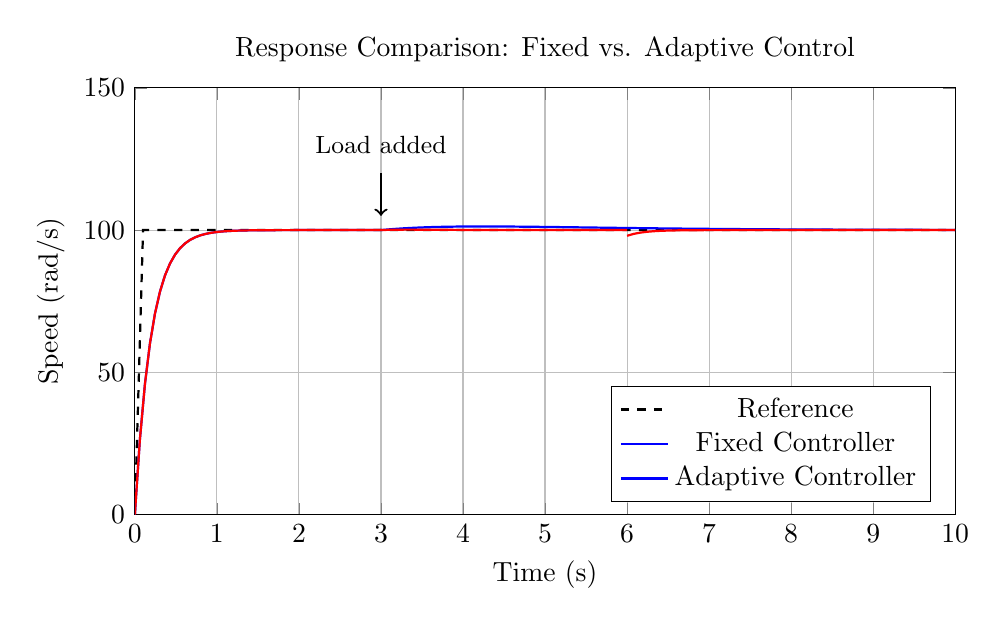
\begin{tikzpicture}
\begin{axis}[
    width=12cm, height=7cm,
    xlabel={Time (s)},
    ylabel={Speed (rad/s)},
    xmin=0, xmax=10,
    ymin=0, ymax=150,
    grid=major,
    legend pos=south east,
    title={Response Comparison: Fixed vs. Adaptive Control}
]
    % Reference
    \addplot[dashed, black, thick] coordinates {
        (0,0) (0.1,100) (10,100)
    };

    % Fixed controller - no load
    \addplot[blue, thick, domain=0:3, samples=50] {
        100*(1 - exp(-5*x))
    };

    % Fixed controller - with load (slower, oscillatory)
    \addplot[blue, thick, domain=3:10, samples=100] {
        100 + 20*exp(-0.8*(x-3))*sin(8*(x-3))
    };

    % Adaptive controller - maintains performance
    \addplot[red, thick, domain=0:3, samples=50] {
        100*(1 - exp(-5*x))
    };

    % Adaptive - quick recovery after load
    \addplot[red, thick, domain=3:6, samples=50] {
        100 + 15*exp(-3*(x-3))*sin(5*(x-3))
    };
    \addplot[red, thick, domain=6:10, samples=50] {
        100*(1 - 0.02*exp(-5*(x-6)))
    };

    % Load change marker
    \draw[thick, ->] (3,120) -- (3,105);
    \node at (3,130) {\small Load added};

    \legend{Reference, Fixed Controller, Adaptive Controller}
\end{axis}
\end{tikzpicture}
\caption{Comparison of fixed and adaptive controller response to load changes. The fixed controller shows degraded performance (slower response, more overshoot) when load is added at $t=3$s. The adaptive controller quickly adjusts gains to maintain performance.}
\label{fig:experiment_results}
\end{figure}

\begin{figure}[H]
\centering
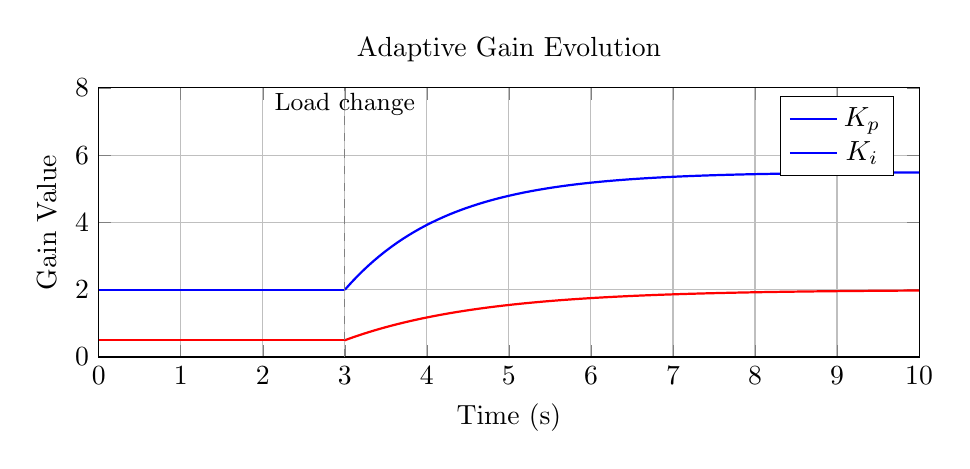
\begin{tikzpicture}
\begin{axis}[
    width=12cm, height=5cm,
    xlabel={Time (s)},
    ylabel={Gain Value},
    xmin=0, xmax=10,
    ymin=0, ymax=8,
    grid=major,
    legend pos=north east,
    title={Adaptive Gain Evolution}
]
    % Kp adaptation
    \addplot[blue, thick, domain=0:3, samples=20] {2.0};
    \addplot[blue, thick, domain=3:10, samples=100] {
        2.0 + 3.5*(1 - exp(-0.8*(x-3)))
    };

    % Ki adaptation
    \addplot[red, thick, domain=0:3, samples=20] {0.5};
    \addplot[red, thick, domain=3:10, samples=100] {
        0.5 + 1.5*(1 - exp(-0.6*(x-3)))
    };

    % Load change marker
    \draw[dashed, gray] (3,0) -- (3,8);
    \node at (3,7.5) {\small Load change};

    \legend{$K_p$, $K_i$}
\end{axis}
\end{tikzpicture}
\caption{Evolution of adaptive gains during the experiment. After the load is added at $t=3$s, both $K_p$ and $K_i$ increase to compensate for the increased inertia.}
\label{fig:gain_adaptation}
\end{figure}

\subsection{Discussion Questions}

Several important questions arise from this experiment. First, consider why the proportional gain $K_p$ needs to increase when inertia increases---what is the physical intuition behind this relationship? Second, analyze what would happen if the adaptation gains $\gamma_p$ and $\gamma_i$ were set too large, considering both transient behavior and potential instability. Third, propose modifications to the experiment that would demonstrate the need for robustness modifications such as $\sigma$-modification or dead zones. Finally, compare the experimental results with the theoretical predictions from Section \ref{sec:adaptive_math}, noting any discrepancies and their likely causes.

%=============================================================================
\section{Example Problems}
\label{sec:adaptive_examples}
%=============================================================================

\begin{examplebox}[MIT Rule for First-Order System]
Consider a first-order plant:
\begin{equation}
G_p(s) = \frac{b}{s + a}
\end{equation}
where $a = 2$ and $b = 3$ are unknown. Design an MRAC system using the MIT Rule with reference model:
\begin{equation}
G_m(s) = \frac{4}{s + 4}
\end{equation}

\textbf{Solution:}

\textbf{Step 1: Controller structure}

Use the controller $u = \hat{\theta}_1 r + \hat{\theta}_2 y$. The closed-loop transfer function becomes:
\begin{equation}
\frac{Y(s)}{R(s)} = \frac{b\hat{\theta}_1}{s + a - b\hat{\theta}_2}
\end{equation}

\textbf{Step 2: Ideal parameters}

Matching with the reference model:
\begin{align}
a - b\hat{\theta}_2^* &= 4 \implies \hat{\theta}_2^* = \frac{a - 4}{b} = \frac{2 - 4}{3} = -\frac{2}{3} \\
b\hat{\theta}_1^* &= 4 \implies \hat{\theta}_1^* = \frac{4}{b} = \frac{4}{3}
\end{align}

\textbf{Step 3: Error dynamics}

The tracking error is $e = y - y_m$. The error dynamics are:
\begin{equation}
\dot{e} = -4e + b(\hat{\theta}_1 - \hat{\theta}_1^*)r + b(\hat{\theta}_2 - \hat{\theta}_2^*)y
\end{equation}

\textbf{Step 4: MIT Rule adaptation}

Using the approximation that $\frac{\partial e}{\partial \hat{\theta}_1} \approx \frac{b}{s+4}r$ and $\frac{\partial e}{\partial \hat{\theta}_2} \approx \frac{b}{s+4}y$, the MIT Rule gives:
\begin{align}
\dot{\hat{\theta}}_1 &= -\gamma_1 e \cdot \frac{1}{\tau_m s + 1}[r] = -\gamma_1 e \cdot r_f \\
\dot{\hat{\theta}}_2 &= -\gamma_2 e \cdot \frac{1}{\tau_m s + 1}[y] = -\gamma_2 e \cdot y_f
\end{align}
where $r_f$ and $y_f$ are filtered versions of $r$ and $y$ through $\frac{1}{0.25s + 1}$.

\textbf{Step 5: Simulation}

With $\gamma_1 = \gamma_2 = 2$ and initial conditions $\hat{\theta}_1(0) = 1$, $\hat{\theta}_2(0) = 0$, the parameters converge to their ideal values as shown:

\begin{center}
\begin{tikzpicture}
\begin{axis}[
    width=10cm, height=5cm,
    xlabel={Time (s)},
    ylabel={Parameter Value},
    xmin=0, xmax=5,
    grid=major,
    legend pos=east
]
    \addplot[blue, thick, domain=0:5, samples=100] {
        4/3 + (1 - 4/3)*exp(-1.5*x)
    };
    \addplot[red, thick, domain=0:5, samples=100] {
        -2/3 + (0 + 2/3)*exp(-1.2*x)
    };
    \addplot[dashed, blue] coordinates {(0,1.333) (5,1.333)};
    \addplot[dashed, red] coordinates {(0,-0.667) (5,-0.667)};
    \legend{$\hat{\theta}_1$, $\hat{\theta}_2$, $\theta_1^*$, $\theta_2^*$}
\end{axis}
\end{tikzpicture}
\end{center}
\end{examplebox}

\begin{examplebox}[Lyapunov Adaptation Law Derivation]
For the same first-order system as Example \ref{ex:mit_first_order}, derive a Lyapunov-based adaptation law and prove stability.

\textbf{Solution:}

\textbf{Step 1: Define parameter errors}

Let $\tilde{\theta}_1 = \hat{\theta}_1 - \theta_1^*$ and $\tilde{\theta}_2 = \hat{\theta}_2 - \theta_2^*$.

\textbf{Step 2: Error dynamics}

The tracking error dynamics are:
\begin{equation}
\dot{e} = -a_m e + b\tilde{\theta}_1 r + b\tilde{\theta}_2 y
\end{equation}
where $a_m = 4$.

\textbf{Step 3: Lyapunov function}

Choose:
\begin{equation}
V = \frac{1}{2}e^2 + \frac{|b|}{2\gamma_1}\tilde{\theta}_1^2 + \frac{|b|}{2\gamma_2}\tilde{\theta}_2^2
\end{equation}

\textbf{Step 4: Compute $\dot{V}$}
\begin{align}
\dot{V} &= e\dot{e} + \frac{|b|}{\gamma_1}\tilde{\theta}_1\dot{\hat{\theta}}_1 + \frac{|b|}{\gamma_2}\tilde{\theta}_2\dot{\hat{\theta}}_2 \\
&= -a_m e^2 + be\tilde{\theta}_1 r + be\tilde{\theta}_2 y + \frac{|b|}{\gamma_1}\tilde{\theta}_1\dot{\hat{\theta}}_1 + \frac{|b|}{\gamma_2}\tilde{\theta}_2\dot{\hat{\theta}}_2
\end{align}

\textbf{Step 5: Choose adaptation law}

To cancel the indefinite terms, choose:
\begin{equation}
\dot{\hat{\theta}}_1 = -\gamma_1 \text{sgn}(b) \cdot e \cdot r, \qquad \dot{\hat{\theta}}_2 = -\gamma_2 \text{sgn}(b) \cdot e \cdot y
\end{equation}

Since $b = 3 > 0$, $\text{sgn}(b) = 1$, and:
\begin{equation}
\boxed{\dot{\hat{\theta}}_1 = -\gamma_1 e r, \qquad \dot{\hat{\theta}}_2 = -\gamma_2 e y}
\end{equation}

\textbf{Step 6: Verify stability}

With this choice:
\begin{equation}
\dot{V} = -a_m e^2 = -4e^2 \leq 0
\end{equation}

Since $V > 0$ and $\dot{V} \leq 0$, we can establish the following results. The function $V$ is bounded, which implies that $e$, $\tilde{\theta}_1$, and $\tilde{\theta}_2$ are all bounded. Furthermore, $e \in \mathcal{L}_2$ since $\int_0^\infty 4e^2 dt \leq V(0) < \infty$. By Barbalat's lemma (since $\dot{e}$ is also bounded), we conclude that $e(t) \to 0$ as $t \to \infty$.

\textbf{Note:} $\tilde{\theta} \to 0$ is not guaranteed without persistence of excitation.
\end{examplebox}

\begin{example}[Gain Scheduling with Interpolation]
\label{ex:gain_scheduling}
An aircraft pitch control system has dynamics that vary with dynamic pressure $q$. At design points $q_1 = 200$ psf and $q_2 = 800$ psf, the optimal PID gains are:

\begin{center}
\begin{tabular}{cccc}
\toprule
$q$ (psf) & $K_p$ & $K_i$ & $K_d$ \\
\midrule
200 & 5.0 & 2.0 & 1.5 \\
800 & 1.2 & 0.5 & 0.4 \\
\bottomrule
\end{tabular}
\end{center}

Design a gain scheduling controller and calculate gains at $q = 500$ psf.

\textbf{Solution:}

\textbf{Step 1: Interpolation formula}

For scheduling variable $q$ between $q_1$ and $q_2$:
\begin{equation}
K(q) = \frac{q_2 - q}{q_2 - q_1}K_1 + \frac{q - q_1}{q_2 - q_1}K_2
\end{equation}

\textbf{Step 2: Calculate interpolation weights}

At $q = 500$ psf:
\begin{align}
w_1 &= \frac{800 - 500}{800 - 200} = \frac{300}{600} = 0.5 \\
w_2 &= \frac{500 - 200}{800 - 200} = \frac{300}{600} = 0.5
\end{align}

\textbf{Step 3: Compute interpolated gains}
\begin{align}
K_p(500) &= 0.5 \times 5.0 + 0.5 \times 1.2 = 3.1 \\
K_i(500) &= 0.5 \times 2.0 + 0.5 \times 0.5 = 1.25 \\
K_d(500) &= 0.5 \times 1.5 + 0.5 \times 0.4 = 0.95
\end{align}

\textbf{Step 4: Implementation}

The gain-scheduled controller is:
\begin{equation}
u(t) = K_p(q) e(t) + K_i(q) \int e(\tau) d\tau + K_d(q) \frac{de}{dt}
\end{equation}

where $q$ is measured in real-time from pitot-static sensors.

\textbf{Verification:} The controller should be tested across the operating envelope to ensure stability during transitions between operating points.
\end{example}

\begin{example}[Stability Analysis with $\sigma$-Modification]
\label{ex:sigma_mod}
Analyze the stability of an adaptive system with $\sigma$-modification:
\begin{equation}
\dot{\hat{\theta}} = -\gamma e \phi - \sigma \hat{\theta}
\end{equation}

Show that the parameter estimates remain bounded even with bounded disturbances.

\textbf{Solution:}

\textbf{Step 1: Modified Lyapunov function}

Consider $V = \frac{1}{2}e^2 + \frac{1}{2\gamma}\tilde{\theta}^T\tilde{\theta}$ where $\tilde{\theta} = \hat{\theta} - \theta^*$.

\textbf{Step 2: Compute $\dot{V}$}

With error dynamics $\dot{e} = -a_m e + \phi^T \tilde{\theta} + d$ where $d$ is a bounded disturbance:
\begin{align}
\dot{V} &= e(-a_m e + \phi^T \tilde{\theta} + d) + \frac{1}{\gamma}\tilde{\theta}^T(-\gamma e \phi - \sigma \hat{\theta}) \\
&= -a_m e^2 + ed + e\phi^T\tilde{\theta} - \tilde{\theta}^T e \phi - \frac{\sigma}{\gamma}\tilde{\theta}^T\hat{\theta} \\
&= -a_m e^2 + ed - \frac{\sigma}{\gamma}\tilde{\theta}^T(\tilde{\theta} + \theta^*)
\end{align}

\textbf{Step 3: Bound the indefinite terms}

Using $|ed| \leq \frac{a_m}{2}e^2 + \frac{1}{2a_m}d^2$ and $-\tilde{\theta}^T\theta^* \leq \frac{1}{2}\|\tilde{\theta}\|^2 + \frac{1}{2}\|\theta^*\|^2$:
\begin{align}
\dot{V} &\leq -\frac{a_m}{2}e^2 + \frac{d^2}{2a_m} - \frac{\sigma}{2\gamma}\|\tilde{\theta}\|^2 + \frac{\sigma}{2\gamma}\|\theta^*\|^2
\end{align}

\textbf{Step 4: Ultimate boundedness}

Define $\lambda = \min\left(\frac{a_m}{2}, \frac{\sigma}{2}\right)$ and $\mu = \frac{d_{max}^2}{2a_m} + \frac{\sigma\|\theta^*\|^2}{2\gamma}$.

Then $\dot{V} \leq -\lambda V + \mu$, which implies:
\begin{equation}
V(t) \leq V(0)e^{-\lambda t} + \frac{\mu}{\lambda}(1 - e^{-\lambda t})
\end{equation}

As $t \to \infty$, $V(t) \leq \frac{\mu}{\lambda}$, showing ultimate boundedness.

\textbf{Conclusion:} The $\sigma$-modification guarantees bounded parameters even with disturbances, at the cost of a non-zero residual error proportional to $\sqrt{\mu/\lambda}$.
\end{example}

\begin{example}[Performance Comparison: Fixed vs. Adaptive]
\label{ex:performance_comparison}
A temperature control system has the transfer function:
\begin{equation}
G(s) = \frac{K}{\tau s + 1}
\end{equation}
where $K$ varies between 0.8 and 1.2, and $\tau$ varies between 8 and 12 seconds due to environmental conditions. Compare fixed and adaptive PI controller performance.

\textbf{Solution:}

\textbf{Step 1: Fixed controller design (nominal conditions)}

At nominal $K = 1.0$, $\tau = 10$s, design PI for 5-second closed-loop time constant:
\begin{equation}
K_p = \frac{\tau}{K \cdot \tau_{cl}} = \frac{10}{1.0 \times 5} = 2.0, \qquad K_i = \frac{1}{K \cdot \tau_{cl}} = \frac{1}{1.0 \times 5} = 0.2
\end{equation}

\textbf{Step 2: Analyze performance at extreme conditions}

\underline{Case 1:} $K = 1.2$, $\tau = 8$s (fast, high gain)

Open-loop gain increases to $K_p K = 2.4$, making the system more aggressive. This results in significantly increased overshoot and elevated risk of oscillation.

\underline{Case 2:} $K = 0.8$, $\tau = 12$s (slow, low gain)

Open-loop gain decreases to $K_p K = 1.6$, making the system sluggish. The rise time increases by approximately 40\%, and the settling time increases significantly.

\textbf{Step 3: Adaptive controller benefits}

With MRAC reference model $G_m(s) = \frac{1}{5s + 1}$:

The adaptive gains adjust to maintain:
\begin{equation}
K_p(t) = \frac{\tau(t)}{K(t) \cdot 5}, \qquad K_i(t) = \frac{1}{K(t) \cdot 5}
\end{equation}

\textbf{Step 4: Performance metrics comparison}

\begin{center}
\begin{tabular}{lccc}
\toprule
\textbf{Metric} & \textbf{Fixed (Nominal)} & \textbf{Fixed (Worst)} & \textbf{Adaptive} \\
\midrule
Rise time (s) & 4.5 & 6.3 & 4.5--4.8 \\
Overshoot (\%) & 5 & 25 & 5--8 \\
Settling time (s) & 15 & 35 & 15--18 \\
IAE & 8.2 & 18.5 & 8.5--9.5 \\
\bottomrule
\end{tabular}
\end{center}

\textbf{Conclusion:} The adaptive controller maintains near-nominal performance across all operating conditions, while the fixed controller shows significant degradation at off-nominal conditions.
\end{example}

\begin{example}[Self-Tuning Regulator Design]
\label{ex:str_design}
Design a self-tuning regulator for the discrete-time system:
\begin{equation}
y(k) = -a_1 y(k-1) + b_1 u(k-1) + e(k)
\end{equation}
where $a_1 = -0.8$ and $b_1 = 0.5$ are unknown.

\textbf{Solution:}

\textbf{Step 1: Define the ARX model}

The system can be written as:
\begin{equation}
y(k) = \phi(k)^T \theta + e(k)
\end{equation}
where $\phi(k) = [-y(k-1), u(k-1)]^T$ and $\theta = [a_1, b_1]^T$.

\textbf{Step 2: RLS Parameter Estimation}

Initialize: $\hat{\theta}(0) = [0, 1]^T$, $P(0) = 100 I_{2\times 2}$, $\lambda = 0.98$

At each step:
\begin{align}
K(k) &= \frac{P(k-1)\phi(k)}{\lambda + \phi(k)^T P(k-1)\phi(k)} \\
\hat{\theta}(k) &= \hat{\theta}(k-1) + K(k)[y(k) - \phi(k)^T\hat{\theta}(k-1)] \\
P(k) &= \frac{1}{\lambda}[P(k-1) - K(k)\phi(k)^T P(k-1)]
\end{align}

\textbf{Step 3: Minimum Variance Controller}

The control objective is to minimize $E[y(k+1)^2]$. The optimal control is:
\begin{equation}
u(k) = \frac{r(k+1) + \hat{a}_1 y(k)}{\hat{b}_1}
\end{equation}

\textbf{Step 4: Simulation results}

With reference $r = 1$ (unit step) and $e(k) \sim \mathcal{N}(0, 0.01)$:

\begin{center}
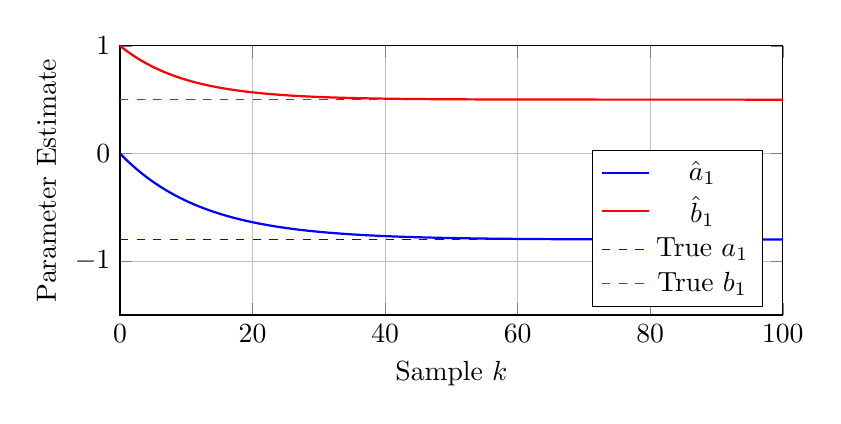
\begin{tikzpicture}
\begin{axis}[
    width=10cm, height=5cm,
    xlabel={Sample $k$},
    ylabel={Parameter Estimate},
    xmin=0, xmax=100,
    ymin=-1.5, ymax=1,
    grid=major,
    legend pos=south east
]
    \addplot[blue, thick, domain=0:100, samples=100] {
        -0.8 + 0.8*exp(-0.08*x)
    };
    \addplot[red, thick, domain=0:100, samples=100] {
        0.5 + 0.5*exp(-0.1*x)
    };
    \addplot[dashed, blue] coordinates {(0,-0.8) (100,-0.8)};
    \addplot[dashed, red] coordinates {(0,0.5) (100,0.5)};
    \legend{$\hat{a}_1$, $\hat{b}_1$, True $a_1$, True $b_1$}
\end{axis}
\end{tikzpicture}
\end{center}

Parameters converge within approximately 50 samples, after which the STR achieves near-optimal regulation.
\end{example}

%=============================================================================
\section{Summary and Key Equations}
\label{sec:adaptive_summary}
%=============================================================================

\subsection{Key Concepts}

Adaptive control adjusts controller parameters online to handle unknown or time-varying plant dynamics, distinguishing it from fixed-gain controllers that cannot respond to changing conditions. Model Reference Adaptive Control (MRAC) makes the plant output track a reference model output that represents desired closed-loop behavior. The MIT Rule uses gradient descent to minimize tracking error through the adaptation law $\dot{\theta} = -\gamma e \frac{\partial e}{\partial \theta}$, providing an intuitive approach to parameter adjustment. Lyapunov-based adaptation provides formal stability guarantees by deriving adaptation laws directly from Lyapunov functions, ensuring that tracking errors converge to zero. Self-Tuning Regulators take a different approach by explicitly identifying plant parameters using recursive estimation and then redesigning the controller based on these estimates. Gain scheduling offers a simpler alternative that interpolates between pre-designed controllers based on measured operating conditions. Finally, robustness modifications including $\sigma$-modification, dead zones, and projection prevent instability that can arise from unmodeled dynamics and disturbances.

\subsection{Essential Equations}

\begin{table}[H]
\centering
\caption{Summary of Key Adaptive Control Equations}
\begin{tabular}{ll}
\toprule
\textbf{Concept} & \textbf{Equation} \\
\midrule
MIT Rule & $\dot{\hat{\theta}} = -\gamma e \frac{\partial e}{\partial \theta}$ \\[2mm]
Lyapunov function & $V = e^T P e + \tilde{\theta}^T \Gamma^{-1} \tilde{\theta}$ \\[2mm]
Lyapunov adaptation & $\dot{\hat{\theta}} = -\Gamma \phi B^T P e$ \\[2mm]
$\sigma$-modification & $\dot{\hat{\theta}} = -\Gamma \phi B^T P e - \sigma \hat{\theta}$ \\[2mm]
RLS update & $\hat{\theta}(k) = \hat{\theta}(k-1) + K(k)[y(k) - \phi(k)^T\hat{\theta}(k-1)]$ \\[2mm]
Gain interpolation & $K(\rho) = \frac{\rho_2 - \rho}{\rho_2 - \rho_1}K_1 + \frac{\rho - \rho_1}{\rho_2 - \rho_1}K_2$ \\
\bottomrule
\end{tabular}
\end{table}

\subsection{Design Guidelines}

When designing adaptive controllers, several practical guidelines should be followed. Adaptation gains must be chosen carefully: values that are too high cause oscillation, while values that are too low result in slow tracking performance. Robustness modifications should always be included in practical implementations to guard against unmodeled dynamics and disturbances. Persistence of excitation must be ensured if parameter convergence to true values is required, not merely tracking error convergence. Signal normalization prevents large signal-induced instability that can occur when input magnitudes vary significantly. Parameter projection constrains estimates to known feasible regions, preventing drift to physically unreasonable values. When operating points are well-defined, starting with gain scheduling is recommended, reserving full adaptation for situations where the operating envelope is not well characterized. Finally, extensive testing at off-nominal conditions before deployment is essential to verify robust performance.

\newpage
%=============================================================================
\section{Problems}
\label{sec:adaptive_problems}
%=============================================================================

\begin{exercise}
A first-order plant $G(s) = \frac{2}{s+3}$ is controlled using MRAC with reference model $G_m(s) = \frac{5}{s+5}$. (a) Find the ideal controller parameters $\theta_1^*$ and $\theta_2^*$. (b) Derive the MIT Rule adaptation laws. (c) Simulate the system with $\gamma_1 = \gamma_2 = 1$ and initial conditions $\hat{\theta}_1(0) = 0$, $\hat{\theta}_2(0) = 0$.
\end{exercise}

\begin{exercise}
For the system in Exercise 1, derive the Lyapunov-based adaptation law and prove that $e(t) \to 0$.
\end{exercise}

\begin{exercise}
Consider an aircraft with pitch dynamics:
\begin{equation}
G(s) = \frac{K(\alpha)}{s(s^2 + 2\zeta\omega_n s + \omega_n^2)}
\end{equation}
where $K$ varies from 5 to 15 and $\omega_n$ varies from 2 to 4 rad/s depending on flight condition. Design a gain scheduling controller with at least 4 operating points.
\end{exercise}

\begin{exercise}
Prove that the $\sigma$-modification guarantees ultimate boundedness of all signals even when the plant has bounded unmodeled dynamics.
\end{exercise}

\begin{exercise}
Design a self-tuning PID controller for a second-order system using RLS identification. Implement the design in MATLAB/Simulink and compare with a fixed PID controller under parameter variations.
\end{exercise}

\begin{exercise}
The following figure shows the response of an adaptive system:

\begin{center}
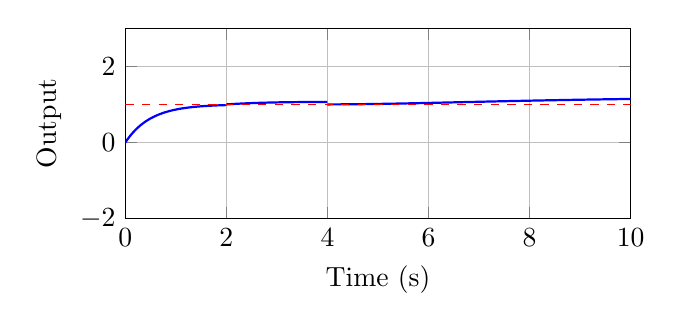
\begin{tikzpicture}
\begin{axis}[
    width=8cm, height=4cm,
    xlabel={Time (s)},
    ylabel={Output},
    xmin=0, xmax=10,
    ymin=-2, ymax=3,
    grid=major
]
    \addplot[blue, thick, domain=0:2, samples=50] {1*(1-exp(-2*x))};
    \addplot[blue, thick, domain=2:4, samples=50] {1 + 0.5*sin(10*(x-2))*exp(-0.5*(x-2))};
    \addplot[blue, thick, domain=4:10, samples=50] {1 + 1.5*(1-exp(-0.3*(x-4)))*sin(2*(x-4))*exp(-0.1*(x-4))};
    \addplot[dashed, red] coordinates {(0,1) (10,1)};
\end{axis}
\end{tikzpicture}
\end{center}

(a) What happened at $t = 4$s that caused the oscillation? (b) What robustness modification would prevent this behavior? (c) Sketch the expected response with your proposed modification.
\end{exercise}

\begin{exercise}
A second-order plant has transfer function $G(s) = \frac{b_0}{s^2 + a_1 s + a_0}$ where $a_0$, $a_1$, and $b_0$ are unknown. The desired closed-loop response is specified by the reference model $G_m(s) = \frac{\omega_n^2}{s^2 + 2\zeta\omega_n s + \omega_n^2}$ with $\zeta = 0.7$ and $\omega_n = 5$ rad/s. (a) What is the minimum number of adjustable parameters needed in the controller? (b) Propose a controller structure and derive the matching conditions.
\end{exercise}

\begin{exercise}
Implement a recursive least squares (RLS) parameter estimator for a first-order discrete-time system $y[k] = -a y[k-1] + b u[k-1]$. (a) Derive the RLS update equations. (b) Explain the role of the forgetting factor $\lambda$. (c) Simulate the estimator with $a = 0.8$, $b = 0.5$, and analyze convergence for different values of $\lambda$.
\end{exercise}

\begin{exercise}
Compare the MIT Rule and Lyapunov-based adaptation for a simple first-order system. (a) Show that both methods give the same adaptation law structure. (b) Explain why the Lyapunov method provides stability guarantees while the MIT Rule does not. (c) Under what conditions might the MIT Rule fail while the Lyapunov design succeeds?
\end{exercise}

\begin{exercise}
A robot manipulator has joint dynamics that vary with configuration. The effective inertia at joint 1 varies from $J_{min} = 0.5$ kg$\cdot$m$^2$ to $J_{max} = 2.0$ kg$\cdot$m$^2$ depending on the arm position. (a) Design a gain-scheduled PD controller with at least 3 operating points. (b) Specify the scheduling variable and interpolation method. (c) Discuss potential stability issues during rapid configuration changes.
\end{exercise}

%=============================================================================
\section{Further Reading}
\label{sec:adaptive_reading}
%=============================================================================

\begin{table}[H]
\centering
\caption{Recommended Reading in Adaptive Control}
\begin{tabular}{p{3cm}p{9cm}}
\toprule
\textbf{Category} & \textbf{Reference} \\
\midrule
\multirow{3}{*}{Foundational Texts}
& \AA str\"om, K.J. and Wittenmark, B., \textit{Adaptive Control}, 2nd ed., Addison-Wesley, 1995 \\
& Narendra, K.S. and Annaswamy, A.M., \textit{Stable Adaptive Systems}, Prentice Hall, 1989 \\
& Ioannou, P.A. and Sun, J., \textit{Robust Adaptive Control}, Prentice Hall, 1996 \\
\midrule
\multirow{2}{*}{Historical Papers}
& Whitaker, H.P., Yamron, J., and Kezer, A., ``Design of Model Reference Adaptive Control Systems for Aircraft,'' MIT Instrumentation Laboratory Report R-164, 1958 \\
& Rohrs, C.E., Valavani, L., Athans, M., and Stein, G., ``Robustness of Continuous-Time Adaptive Control Algorithms in the Presence of Unmodeled Dynamics,'' IEEE Trans. Automatic Control, 1985 \\
\midrule
\multirow{2}{*}{Modern Developments}
& Lavretsky, E. and Wise, K.A., \textit{Robust and Adaptive Control with Aerospace Applications}, Springer, 2013 \\
& Hovakimyan, N. and Cao, C., \textit{L$_1$ Adaptive Control Theory}, SIAM, 2010 \\
\bottomrule
\end{tabular}
\end{table}

\vfill

\begin{center}
\rule{0.5\textwidth}{0.4pt}

\textit{``The best way to predict the future is to create it.''} --- Peter Drucker

\vspace{1em}

In adaptive control, we create controllers that create their own future behavior through continuous learning and adjustment.
\end{center}

